\documentclass[conference]{IEEEtran}
\IEEEoverridecommandlockouts
% The preceding line is only needed to identify funding in the first footnote. If that is unneeded, please comment it out.
\usepackage{cite}
\usepackage{amsmath,amssymb,amsfonts}
\usepackage{algorithmic}
\usepackage{graphicx}
\usepackage{textcomp}
\usepackage{xcolor}
\def\BibTeX{{\rm B\kern-.05em{\sc i\kern-.025em b}\kern-.08em
    T\kern-.1667em\lower.7ex\hbox{E}\kern-.125emX}}
\begin{document}

\title{Data-Driven Recommendation of Academic
Options Based on Personality Traits\\
% {\footnotesize \textsuperscript{*}Note: Sub-titles are not captured in Xplore and
% should not be used}
\thanks{Identify applicable funding agency here. If none, delete this.}
}
% https://www.overleaf.com/project/621d7856db9f84677f85dda0
\author{\IEEEauthorblockN{Aashish Ghimire}
\IEEEauthorblockA{\textit{Department of Computer Science} \\
\textit{Utah State University}\\
Logan, Utah \\
aashish.ghimire@usu.edu}
\and
\IEEEauthorblockN{Travis Dorsch}
\IEEEauthorblockA{\textit{Department of Human Development and Family Studies} \\
\textit{Utah State University}\\
Logan, Utah \\
travis.dorsch@usu.edu}
\and
\IEEEauthorblockN{John Edwards}
\IEEEauthorblockA{\textit{Department of Computer Science} \\
\textit{Utah State University}\\
Logan, Utah \\
john.edwards@usu.edu}
% \and
% \IEEEauthorblockN{4\textsuperscript{th} Given Name Surname}
% \IEEEauthorblockA{\textit{dept. name of organization (of Aff.)} \\
% \textit{name of organization (of Aff.)}\\
% City, Country \\
% email address or ORCID}
% \and
% \IEEEauthorblockN{5\textsuperscript{th} Given Name Surname}
% \IEEEauthorblockA{\textit{dept. name of organization (of Aff.)} \\
% \textit{name of organization (of Aff.)}\\
% City, Country \\
% email address or ORCID}
% \and
% \IEEEauthorblockN{6\textsuperscript{th} Given Name Surname}
% \IEEEauthorblockA{\textit{dept. name of organization (of Aff.)} \\
% \textit{name of organization (of Aff.)}\\
% City, Country \\
% email address or ORCID}
}

\maketitle

\begin{abstract}
The choice of academic major and academic institution has a large effect on a person's career. About 40\% of students either transfer to a different major or different college or drop out of college within six years. Various social science research has shown that personality traits play a significant role in academic preference. Still, there has not been a comprehensive, data-driven approach to translate this into academic choice. In light of this gap in understanding, we surveyed over 500 people between 18 and 25 years old to capture personality traits and preference of college major and used that information to train a machine learning model to predict college major preference. This research validates the viability of using personality traits as indicators for educational preference. We demonstrate that using a decision tree model, accurate classification can be done, with over 90\% accuracy. Furthermore, we explored the two methods of dimension reduction - one using Principal Component Analysis (PCA) and another relying on Social Science research on the Big-Five personality Traits (also known as OCEAN indices) to simplify the problem further. With these techniques, the dimension was reduced by half without decreasing the accuracy of our classifier. We compared other popular machine learning methods and demonstrated that a decision tree is best for such an application. With this research, a readily deployable recommendation system was created that can help students find their most enjoyable academic path and aid guidance counselor and parents with their recommendations.

\end{abstract}

\begin{IEEEkeywords}
classification, principal component analysis(pca), personality types, academic preference 
\end{IEEEkeywords}



%%%%%%%%%%%%%%%%%%%%%%%%%%%%%%%%%%%%%%%%%%%%%%%%%%%%%%%%%%%%%%
\section{Introduction}

The choices of academic major and institution are among the most fundamental steps in a person’s career. A student typically makes that decision during their high school years and often without sufficient information. According to the department of education, the overall 6-year graduation rate for first-time, full-time undergraduate students who began seeking a bachelor’s degree at 4-year degree-granting institutions in fall 2012 was 62 percent. That is, by 2018, some 62 percent of students had completed a bachelor’s degree at the same institution where they started in 2012. The 6-year graduation rate was 61 percent at public institutions, 67 percent at private nonprofit institutions, and 25 percent at private for-profit institutions \cite{hussar2020condition}. This 6- year limit does not include the breaks taken for military service, religious service, etc. For the cohort starting in 2011, the eight-year graduation rate was only 61.8 percent \cite{nscr}.
Traditionally, schools provide a guidance counselor to help students make these decisions. According to The National Association for College Admission Counseling (NACAC), the national student-to-counselor ratio is 482:1. In some states like Arizona, there are as many as 924 students per guidance counselor \cite{american2015state}. At this ratio, a guidance counselor cannot realistically suggest the best-fit college or major for each student. In order to aid these students with making those decisions, guidance counselors could potentially use a data-driven approach. As of now, the state-of-the-art guidance counselor tool is the college database that can be used to filter the institution based on size, location, major, etc., but there is little beyond that, according to market research done by Graphium, Inc.~\cite{ghimire2019graphium}. There are some commercial services available directly to students based on their preferences, but
they are riddled with university advertisements and sponsored sections, where colleges that pay are boosted higher up on the chart and are not very distinguishable from the real recommendation.

% (Examples include niche.com, unigo.com, etc.) Similarly, The College Board – the most popular college recommendation website – is run by the same institution that conducts SAT tests. It puts the full weight on college test scores and GPA but not the strengths, weaknesses, and personality of the students.

There have been several studies to classify human traits into different personality types and to study student performance in different academic majors. Most famously, Holland \cite{schneider1983holland} classified academic major with six personality types. The analysis of covariance results indicated that four of the five expectation scales were significantly related to students’ personality types. In contrast, only two of the expectation scales were significantly related to environment types. This classification has been widely used across different papers in psychology research for decades \cite{Weidman2005}. Allred et al. studied the validity of the stereotypes surrounding the choice of academic majors and stress level in different academic disciplines \cite{allred2013relationship}. Most of these findings are from qualitative studies that do not use a data driven approach to validate their conclusions.
In building on these findings, our study was designed to answer three research questions:
\begin{itemize}
    \item R1: How effective is the use of personality traits in predicting a preferred college major?
    \item R2: How do expert-derived personality traits compare to a data-driven dimension reduction technique?
    \item R3: What are the unique personality traits found in students preferring different majors?
\end{itemize}



%%%%%%%%%%%%%%%%%%%%%%%%%%%%%%%%%%%%%%%%%%%%%%%%%%%%%%%%%%%%%%
\section{Methods}

Since there is no publicly available dataset suitable for classifying a student’s preference of major based on their personality, we, as a major part of this study, collected such a dataset in the form of a survey. This survey asked ten probing personality questions, as listed below. It also asked three questions related to college major preference, along with demographics questions. Utilizing survey responses, the scores for five personality traits derived from the ten personality questions were used to calculate 5-dimensional personality features using the OCEAN model. For comparison, we also built classification models using 5-dimensional personality featured from the ten personality questions using Principal Component Analysis (PCA). In the present study, we compare the performance of the expert-derived OCEAN personality traits with PCA-derived traits.

\subsection{Ten-Item Personality Inventory (TIPI) - 10 Questions for the Personality Type Classification}\label{subsec2}
In the user survey, the following ten questions \cite{gosling2003very} were asked to gauge the personality type of the user. Each answer is on a seven-level Likert scale:
\begin{itemize}
    \item TP 1: I see myself as extroverted and enthusiastic.
    \item TP 2: I see myself as critical and quarrelsome.
    \item TP 3: I see myself as dependable and self-disciplined.
    \item TP 4: I see myself as anxious and easily upset.
    \item TP 5: I see myself as complex \& open to new experiences.
    \item TP 6: I see myself as reserved and quiet.
    \item TP 7: I see myself as sympathetic and warm.
    \item TP 8: I see myself as disorganized and careless.
    \item TP 9: I see myself as calm and emotionally stable. 
    \item TP 10: I see myself as conventional and uncreative.

\end{itemize}

\subsection{Big Five Personality Traits (OCEAN) for dimension reduction}\label{subsec2}
For classifying the user and better understanding their personality type, we use the Big Five Personality Trait index \cite{john1991big}. The five traits are openness, conscientiousness, extraversion, agreeableness, and neuroticism. This is often referred as the OCEAN index. In our study, each trait was classified as either negative (score of 2.5 or under), neutral (between 2.5 to 5.5) or positive (5.5 and over). These three buckets of being negative, neutral, or positive in each of the five personality traits gives interpretable categories that can be used to
provide personalized guidance to the students.
There are certain connotations based on a
personality type being positive or negative. If
the user is in the neutral bucket, no inference is
made from that index. 

% A brief introduction of
% those five personality types and the connotation
% associated with each bucket of those traits are
% described in the Table 2 as described by
% Barrick and Mount (1991).



\subsection{Calculations of the mean OCEAN scores}\label{subsec2}

A seven-level Likert Scale \cite{joshi2015likert} was used to record the responses to the ten questions on the personality of TIPI (see section 3.1). This is the recommended scoring method by the creator of TIPI \cite{gosling2003very}.
Scores for the OCEAN personality index can be from the ten scores of the TIPI. Scores for each of the five OCEAN categories are calculated using the following formulae as per the Gossling et. al., where TQ1, TQ2 ... TQ10 refer to answers to the 10 TIPI personality questions. Those formulae are shown in \ref{eq1}, \ref{eq2}...\ref{eq5}.

\begin{equation}
% \label{eqn:Equation to calculate TIPI Socre}
Openness = \frac{\text{TP5 + (8 - TP10)}}{2}
\label{eq1}    
\end{equation}

\begin{equation}
Conscientiousness = \frac{\text{TP1 + (8 - TP8)}}{2} 
\label{eq2}    
\end{equation}

\begin{equation}
Extraversion = \frac{\text{TP1 + (8 - TP6)}}{2}
\label{eq3}    
\end{equation}

\begin{equation}
Agreeableness = \frac{\text{ (8 - TP2) + TP7}}{2}
\label{eq4}    
\end{equation}

\begin{equation}
Neuroticism = \frac{\text{(8 - TP4) + TP9 }}{2}
\label{eq5}    
\end{equation}

%%%%%%%%%%%%%%%%%Not Showing Connotations 
\iffalse
\subsection{Personality Traits Connotations}\label{subsec2}
Different positive and negative connotation associated with each personality type are listed in the Table \ref{table:ptraits} as described by Brick et al. \cite{bruck2003relationship}. 



\begin{table}
\begin{tabular}{|p{2.3cm}|p{4.2cm}|p{4.2cm}|}
\hline
Personality Traits & Positive (\textgreater{}= 5.5) & Negative (\textless{}=2.5) \\
\hline
Openness           & imagination, training performance, academic achievement, cognitive functioning, creative achievement, independence & training performance (negative), academic achievement (negative), practicality, conformity, negative affect, stress \\ \hline
Conscientiousness  & job performance, academic Achievement motivation, judgement, health, stress (negative),  problem-solving, goal-orientation, longevity & job performance (negative), academic achievement (negative), impulsivity, carelessness, cognitive decline \\ \hline
Extraversion       & teamwork, affection, relationship satisfaction, positive affect, well-being & teamwork (negative), reservations, somber \\ \hline
Agreeableness      & positive relations with others, job performance, academic achievement, softhearted, generosity, altruism, relationship satisfaction, positive emotions & negative relations with others, job performance (negative), academic achievement (negative), uncooperative, skepticism \\ \hline
Neuroticism        & teamwork (negative), insecurity, health risk, low well-being in late adulthood & teamwork, satisfaction \\ \hline
\end{tabular}
\label{table:ptraits}
\caption{Connotation associated with being in different personality traits score.}
\end{table}
\fi
 
%%%%%%%%%%%%%%%%%%%%%%%%%%%%%%%%%%%End of Block Comment %%%%%%%%%%%%%%%%%%%%%%%%%%%%%%%%%%%%%%%%%% 
%  \begin{center}
% \hline
% \begin{tabular}{|c|}

% \end{tabular}
% \end{center}


\subsection{Academic Major Preference}\label{subsec2}
The list of all college majors listed by the US Department of education was obtained from their public database \cite{doe}. This yielded 397 unique majors. To narrow the list, only majors offered at more than 100 schools were picked, which left 261 majors. From there, we divided the majors into 14 general categories based on how these majors are commonly classified in their school’s organization structure. These are shown in Table \ref{table:majorcat}.
After asking three demographics and ten personality questions, survey takers were provided with an attention check question such as “what is 2 + 2?”. After passing the attention checker, users were provided the question where they were presented a list of five academic majors randomly selected from the 14 major categories and asked to
choose the major that interests them the most. An example of a question regarding the academic major in the survey is shown below:\\


\hline 
\vspace{8pt}
Of the college majors shown below, select the one that interests you the most: 
\begin{itemize}
\item Language and Literature (Literature, English, Foreign Language, etc.) 
\item Life Science (Biology, Ecology, Neuroscience, etc) 
\item Education (Elementary Education, Special Ed and Teaching, Curriculum Development, etc) 
\item Health Services (Medical Doctor, Nursing, Dental, etc) 
\item Management (Business Administration, Finance, Management Science, etc) 
\vspace{8pt}
\end{itemize}
\hline 


% \begin{figure}[h]
% 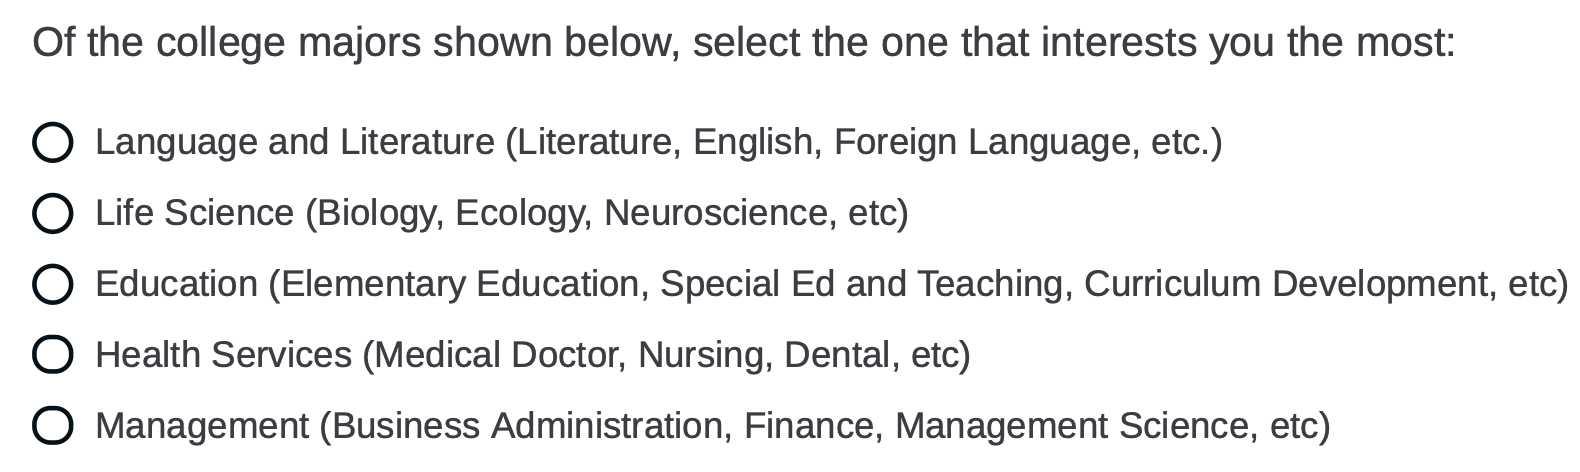
\includegraphics[scale=0.2]{figs/majq.png}
% \caption{Example of question asking user for their preferred major}
% \label{fig:majq}
% \centering
% \end{figure}


\begin{table}[]
\centering
\begin{tabular}{|l|l|}

\hline
{  Categories}                     & \# of majors included  \\ \hline
{  Management}                     & {  29}                                                                       \\ \hline
{  Business}                       & {  13}                                                                       \\ \hline
{  Health Service}                 & {  25}                                                                       \\ \hline
{  Law / Administration}           & {  15}                                                                       \\ \hline
{  Education}                      & {  10}                                                                       \\ \hline
{  Engineering}                    & {  46}                                                                       \\ \hline
{  Social and Behavioural Science} & {  21}                                                                       \\ \hline
{  Life Science}                   & {  30}                                                                       \\ \hline
{  Language and Literature}        & {  16}                                                                       \\ \hline
{  Vocational}                     & {  16}                                                                       \\ \hline
{  Arts}                           & {  9}                                                                        \\ \hline
{  Communication \& Media}         & {  8}                                                                        \\ \hline
{  Physical Science}               & {  16}                                                                       \\ \hline
{  Philosophy \& Theology}         & {  10}                                                                                        \\ \hline
\end{tabular}
\vspace{4pt}
\caption{Table showing the number of majors in each general major category}
\label{table:majorcat}
\end{table}

\subsection{Survey Platform and Data Collection}\label{subsec2}
The survey was designed using Qualtrics’s survey platform. Survey responses were collected from two different sources: Utah State University and Amazon Mechanical Turk (MTurk) workers. For the sake of comparison, these two groups of data were analyzed and used separately. Our Institutional Review Board (IRB) approved the surveys for both Utah State University students and MTurk workers with the questionnaire varied slightly to fit the logistics of validating and paying MTurk’s respondents. All participants were compensated with one dollar in the form of Amazon gift card.

\subsubsection{Survey of students at Utah State University}\label{subsubsec2}
Our survey was completed by students at Utah State University. A Quick Response (QR) Code linked to the survey was emailed to the cadets of the US Army Reserves Officer Training Corps (ROTC) program at the University. The QR code was also sent by a Teaching Assistant to students in a General Psychology class at USU. The age of the respondents was restricted to 25 and under.

\subsubsection{Survey using Amazon Mechanical Turk (MTurk) platform}\label{subsubsec2}
The MTurk platform was used to gather additional survey results. MTurk is a commercial survey and crowd-sourcing platform where users are compensated for completing tasks. Using MTurk’s filter feature, we restricted the respondents to only United States residents. Similarly, the survey was only made available to users with at least a High School diploma using MTurk’s premium filter purchase. To avoid spam responses, Amazon provides an option to limit the exposure of the surveys to a set of reliable survey takers. The reliability of survey takers is generally measured in terms of acceptance rate. MTurk allows the survey requester to accept or reject surveys based on the quality of work. For example, if a user tends to complete surveys in a very short time, or they use other programmatic tools to complete it, they get rejected more often and have a lower acceptance rate. For the purpose of this study, MTurk filter was used
to limit responses to users with more than 95\% acceptance rate and 500 accepted surveys.

%%%%%%%%%%%%%%%%%%%%%%%%%%%%%%%%%%%%%%%%%%%%%%%%%%%%%%%%%%%%%%%%%%




\section{Survey Results}
\subsection{Survey Participation: Amazon Mechanical Turk}\label{subsec3}


There were a total of 728 responses from Amazon Mechanical Turk, of which 420 who
fully completed the survey were aged between 18 to 25. We next looked into the completion
time and removed any surveys that took less than 60 seconds. 355 responses remained after this
filter. Among these 355 responses, the mean completion time was 142 seconds, and the median
was 106 seconds.

\subsubsection{Gender distribution}\label{subsubsec3}
In the MTurk survey, as shown in Table \ref{table:mtgender}, survey participant are fairly even in gender distribution as compared to USU data.

\begin{table}
\centering
\begin{tabular}{|l|c|c|}
% \toprule
\hline
Gender     & MTurk Count & USU Count \\
\hline

% \midrule
Male       & 176 & 36  \\
Female     & 171 & 151  \\
Non-Binary & 8  & 1   \\
\hline

% \bottomrule
\end{tabular}
\vspace{4pt}
\caption{Gender distribution of participant in MTurk and USU data.}
\label{table:mtgender}
\end{table}

\subsubsection{Race distribution}\label{subsubsec3}

The race distribution of survey is as listed in Table \ref{table:mtrace}.
The MTurk distribution is not far off from the United State's national race distribution according to the United States Census Bureau \cite{uscensus}. 


\begin{table}
\centering
\begin{tabular}{|l|c|c|c|c|}
% \toprule
\hline
                                          & MTurk && USU &\\
Race                                      & Count & MTurk \% & Count & USU \% \\
\hline
% \midrule
White                                     & 266 & 75\% & 164 & 87.23\% \\
Black or African American                 & 44 & 12.67\%  & 2 & 1.06\% \\
American Indian/Alaska Native          & 3  & 0.8\% & 3 & 1.59\%  \\
Asian                                     & 41  & 11.54\% & 15 & 7.97\%  \\
Native Hawaiian/Pacific Islander & 1 & 0.28\% &  1 &  0.53\%  \\
Others                                    & 11  & 3.09\% & 3 & 1.59\%  \\
% \bottomrule
\hline
\vspace{4pt}
\end{tabular}
\caption{Race distribution of  participant in Mturk and USU data.}
\label{table:mtrace}
\end{table}


\subsection{Survey Participation : Utah State University}\label{subsec3}
There were a total of 204 responses from Utah State University. However, when we select only those who are aged between 18 to 25 and fully completed the survey, we have 195 left. We next looked into the completion time and removed the surveys that took less than 60 seconds. After these filter criteria, 188 responses remained. For that valid data, the mean completion time is 221 seconds, and the median is 146 seconds. 

\subsubsection{Sampling Bias and separate processing of data:}\label{subsubsec3}
As per most research done among two different communities, this survey is vulnerable
to a sampling bias. The US population is about 13.4\% Black or African American
(Bureau, 2016), but the proportion in Utah State University’s survey is under 1%. While
this is closer to Utah State’s population (1.5\%). The racial composition is MTurk’s data is much closer to the US
demography. For example, it has about 12.
5\% of Black or African American population
- very similar to national averages.
MTurk’s data is well balanced in terms of gender, while USU’s survey is skewed
towards higher female participation. In terms of time taken to complete the survey, USU
has a much higher time (mean of 221 seconds as opposed to 142 seconds at MTurk).
USU participants were guaranteed to be students, but the same could not be said for the
MTurk survey.

\section{Classification Results}\label{sec4}
Our first research question (R1) is: How effective is the use of personality traits
in predicting a preferred college major? To answer this question, we built a machine
learning model (specifically, a decision tree) to predict a students’ preferred academic
major based on their personality type. We built models using different feature vectors.
The first is raw 10-question personality type. The second is 5 dimensional OCEAN
index and the third is the 5-dimensional index derived from Principal Component
Analysis (PCA). Using these different feature sets allowed us to objectively judge the
quality of the widely accepted OCEAN index and answer our second research question
R2: How do expert-derived personality traits compare to a data-driven dimension
reduction technique? Furthermore, using the decision tree classification model with its
high degree of interpretability helps us answer our third research question R3: What are
the unique personality traits found in students preferring different majors?

\subsection{ Classification based on raw TIPI survey}\label{subsec4}
For the first part of the classification, the 10-dimensional raw inputs from users
were used as features. Decision trees natively support multi-class prediction, which is
convenient because our target variable, preferred major, could be one of 14 general
categories of academic majors.
Since each user was asked for their preferred major three times, there are three answers
for each participant. The Scikit-learn \cite{scikit-learn} library was used for
decision-tree classification. The features and target are as shown in \ref{table:rawclf}.



\begin{table}[h]
\begin{tabular}{|l|l|}
\hline
Feature List    & Target                                                                                       \\ \hline
\begin{tabular}[c]{@{}l@{}}gender,\\ 10 questions \\asked for \\personality traits\\ questionnaire\end{tabular} & \begin{tabular}[c]{@{}l@{}}Management, Business,Health Service,\\ Law / Administration, Education,\\ Engineering, Social and Behavioural Science,\\ 
Life Science,  Language and Literature,\\ Vocational, Arts, Communication \& Media,\\ 
Physical Science, Philosophy \& Theology \end{tabular} \\ \hline
\end{tabular}
\vspace{4pt}
\caption{Features and target class for classification with raw TIPI survey responses }
\label{table:rawclf}
\end{table}
% \usepackage{array}
% % \documentclass{article}
% \begin{center}
% \begin{tabular}{|m{5em} |m{5em}| } 
%  \hline
%  Feature List & Target  \\ 
%   \hline
%  gender, 10 questions asked for  personality traits questionnaire & Management, Business, Health Service, Law Administration, Education, Engineering, Social and Behavioural Science, Life Science,  Language and Literature, Vocational, Arts, Communication \& Media, Physical Science, Philosophy \& Theology  
%  \hline
% \end{tabular}
% \end{center}
% \end{document}

%%%%%%%%%%%%%Only showing sample of two figure for page reasons %%%%%%%%%%%%%%%%%%

% The normalized distribution of college majors preference in the MTurk survey based on
% the positive and negative responses on openness, conscientiousness, extraversion,
% agreeableness and neuroticism, and are shown in Figure 3 through 7 respectively.
% Neutral responses are not shown.


A sample result of normalized distribution of college majors preference in the MTurk survey based on
the positive and negative responses on conscientiousness is shown in figure \ref{fig:c}. Neutral responses and other personality types are not shown.


%%%%%%%%%%%%%%%%%%%%%%%%%%%%%%%%%%%%%% ^^^ %%%%%%%%%%%%%%%%%%%%%%%%%%%%%%%%%%%

% \begin{figure}[h]
% \includegraphics[scale=0.4]{figs/o.png}
% \caption{Distribution of college majors based on Openness using results from the MTurk Survey}
% \label{fig:o}
% \centering
% \end{figure}

\begin{figure}[h]
\includegraphics[scale=0.4]{figs/c.png}
\caption{Distribution of college majors based on Conscientiousness  using results from the MTurk Survey}
\label{fig:c}
\centering
\end{figure}

% \begin{figure}[h]
% \includegraphics[scale=0.4]{figs/e.png}
% \caption{Distribution of college majors based on Extraversion  using results from the MTurk Survey}
% \label{fig:e}
% \centering
% \end{figure}

% \begin{figure}[h]
% \includegraphics[scale=0.4]{figs/a.png}
% \caption{Distribution of college majors based on Agreeableness using results from the MTurk Survey}
% \label{fig:a}
% \centering
% \end{figure}

% \begin{figure}[h]
% \includegraphics[scale=0.4]{figs/n.png}
% \caption{Distribution of college majors based on Neuroticism  using results from the MTurk Survey}
% \label{fig:n}
% \centering
% \end{figure}


\subsubsection{Tree depth and classification}\label{subsubsec2}
The decision tree is affected by the depth of the tree – so we benchmarked with
trees of depth ranging from 1 to 100 levels. This allows for finding the optimal tree
depth. Figure 8 shows the accuracy of classification over different depths of decision
tree and using different feature sets. The red graph is using raw answers, which
generally performs the best.
From Figure  \ref{fig:USUall3} we can see that the decision tree performs well at a depth of 16 with an
accuracy of 0.959. While the accuracy may slightly increase for a higher depth of tree,
we want to keep the tree as shallow as possible to ensure that the model does not suffer
from overfitting, thus keeping the model generalizable.

\begin{figure}[h]
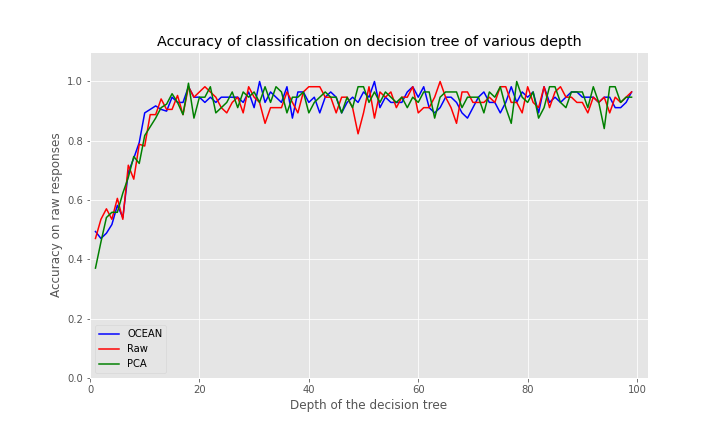
\includegraphics[scale=0.4]{figs/USUall3.png}
\caption{Accuracy of the different decision tree over different tree depth}
\label{fig:USUall3}
\centering
\end{figure}

\subsection{Dimension Reduction - by OCEAN Indexes}\label{subsec4}
For larger datasets, using the answer of each TIPI questionnaire as the feature
set to train the classifier is often time consuming and unnecessary. This can be done
with similar accuracy using dimension reduction. Much of the time in machine learning,
dimension reduction is a black box, and the feature sets derived from higher dimensions
to lower dimensions have no intuitive real-world meaning. The OCEAN Index,
however, reduces 10 TIPI questions to 5 interpretable attributes.
From Figure \ref{fig:USUall3}, the decision tree performs well at a depth of 17 with an accuracy of 0.92
and later at depth 20 with an accuracy of 0.95. Here we can see that the number of
feature sets was cut in half; however, the accuracy is still very close to when compared
with using the raw data.

\begin{figure}[h]
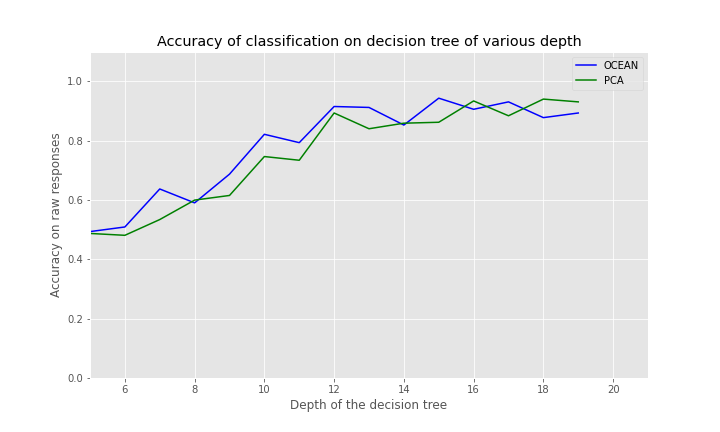
\includegraphics[scale=0.35]{figs/zoomed2.png}
\caption{Accuracy of OCEAN and PCA technique between depth 5-20.}
\label{fig:zoomed2}
\centering
\end{figure}

\subsection{Dimension Reduction by Principal Component Analysis}\label{subsec4}
For the third technique after raw TIPI scores and OCEAN dimension reduction,
Principal Component Analysis (PCA) was used for reducing the dimension of user
responses into five components. Unlike OCEAN, these components do not have a real-world meaning.
The data was first fit into PCA to get the first five principal components. Scikit-learn
was used for decision-tree classification.
The decision tree is also affected by the depth of the tree - hence it is benchmarked with
trees of depth 1 to 100 level. This allows for finding the optimal tree depth. Figure \ref{fig:zoomed2}
shows the accuracy of classification over different depth of the decision tree.

\subsection{Unique personality traits found in students preferring different majors}\label{subsec4}
From the study, we were able to see the difference in different personality traits
in students preferring each academic majors. For example, in figure \ref{fig:score_o}, Business
majors have the lowest “openness” score while philosophy and theology majors have
the highest openness scores. This makes intuitive sense, as theology and philosophy
majors are expected to deal with the wide range of views and people. 


%%%%%%%%%%%%%. Show the remaining figures in the long version of paper online/ redirect to websites? %%%%%%

% The distribution for each of traits conscientiousness, extraversion, agreeableness and neuroticism for all
% majors are presented in Figures \ref{fig:score_o} through \ref{fig:score_n}.

  The distribution for openness score for each major categories is presented in figure \ref{fig:score_o}. 
  % through \ref{fig:score_n}.

\begin{figure}[h]
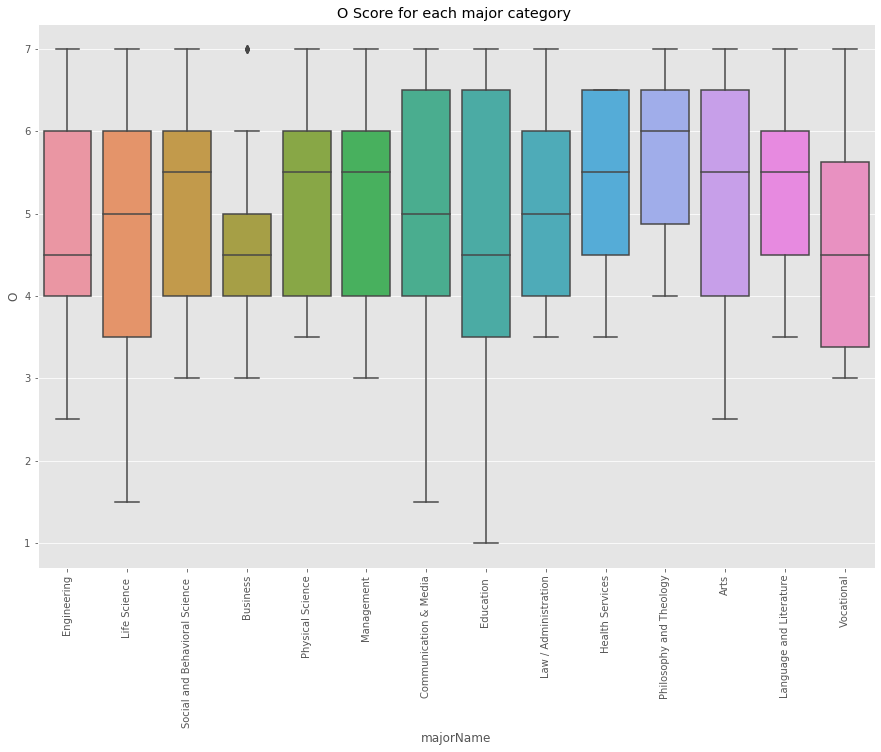
\includegraphics[scale=0.28]{figs/score_o.png}
\caption{Distribution of "Openness" traits among different academic majors.}
\label{fig:score_o}
\centering
\end{figure}

% \begin{figure}[h]
% 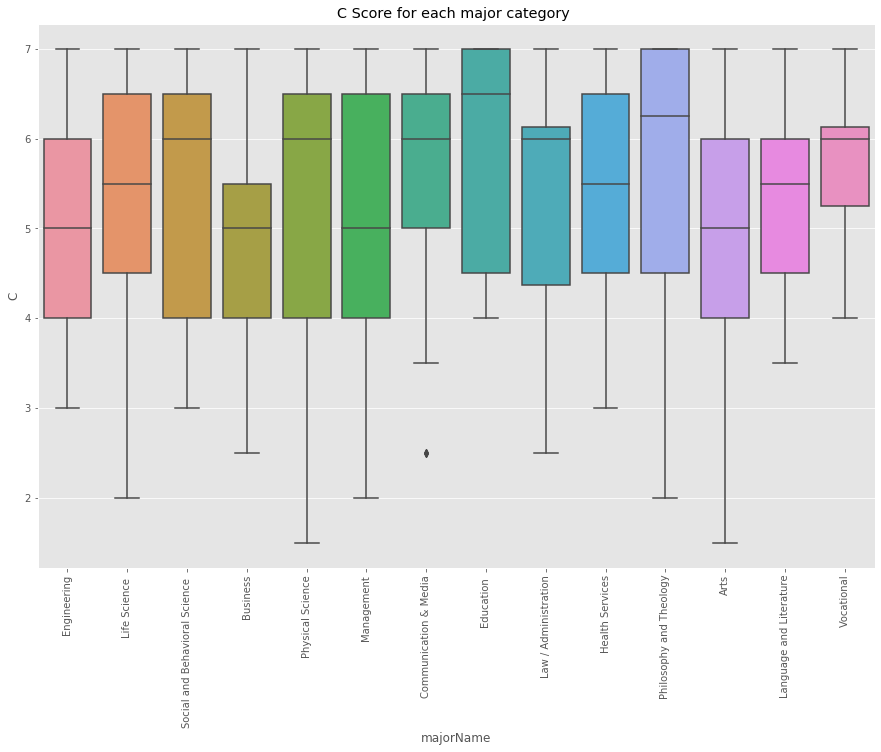
\includegraphics[scale=0.25]{figs/score_c.png}
% \caption{Distribution of "Conscientiousness" traits among different academic majors.}
% \label{fig:score_c}
% \centering
% \end{figure}

% \begin{figure}[h]
% 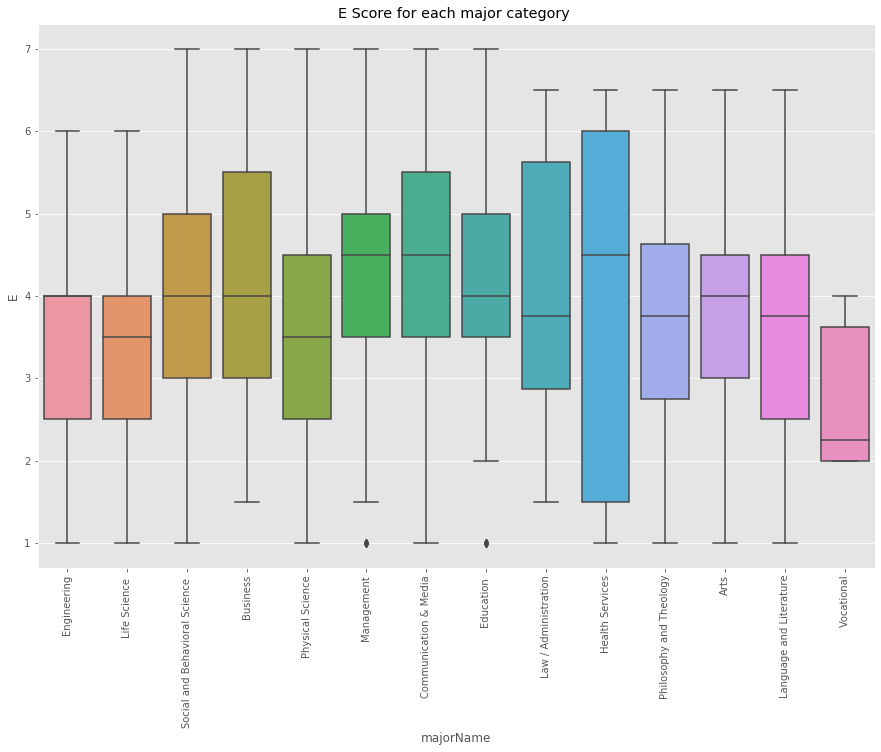
\includegraphics[scale=0.25]{figs/score_e.png}
% \caption{Distribution of "Extraversion" traits among different academic majors.}
% \label{fig:score_e}
% \centering
% \end{figure}

% \begin{figure}[h]
% 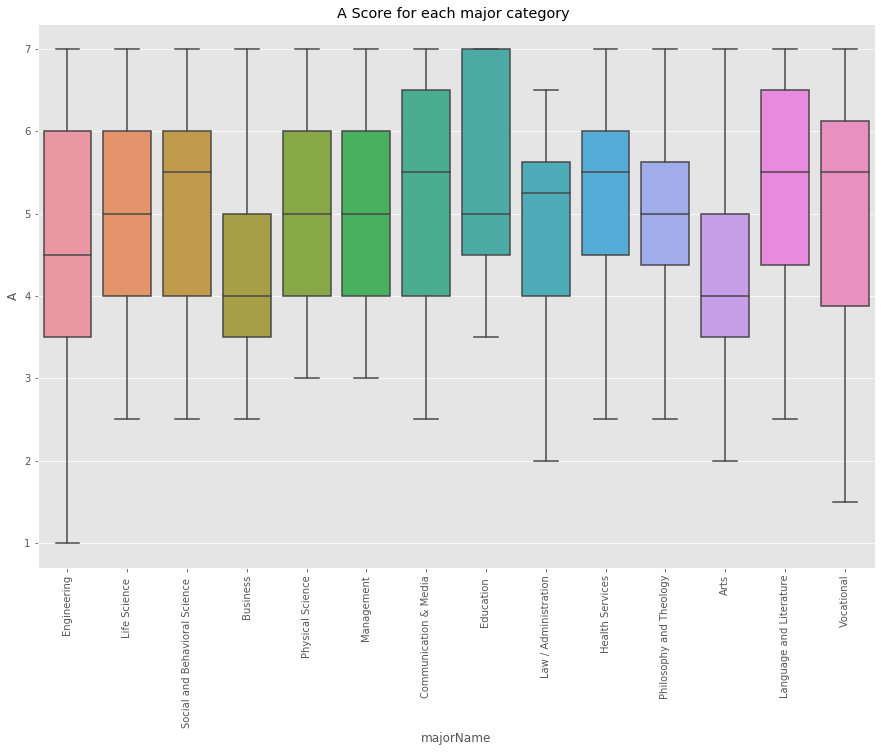
\includegraphics[scale=0.25]{figs/score_a.png}
% \caption{Distribution of "Agreeableness" traits among different academic majors.}
% \label{fig:score_a}
% \centering
% \end{figure}

% \begin{figure}[h]
% 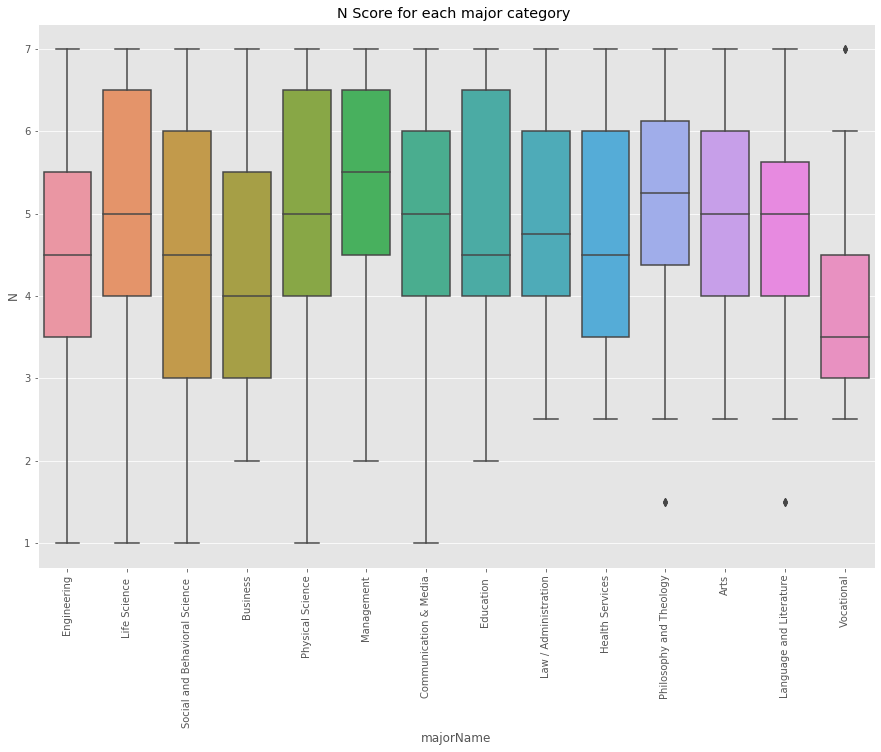
\includegraphics[scale=0.245]{figs/score_n.png}
% \caption{Distribution of "Neuroticism" traits among different academic majors.}
% \label{fig:score_n}
% \centering
% \end{figure}

% \section*{Acknowledgment}

% The preferred spelling of the word ``acknowledgment'' in America is without 
% an ``e'' after the ``g''. Avoid the stilted expression ``one of us (R. B. 
% G.) thanks $\ldots$''. Instead, try ``R. B. G. thanks$\ldots$''. Put sponsor 
% acknowledgments in the unnumbered footnote on the first page.

% \section*{References}

% Please number citations consecutively within brackets \cite{b1}. The 
% sentence punctuation follows the bracket \cite{b2}. Refer simply to the reference 
% number, as in \cite{b3}---do not use ``Ref. \cite{b3}'' or ``reference \cite{b3}'' except at 
% the beginning of a sentence: ``Reference \cite{b3} was the first $\ldots$''

% Number footnotes separately in superscripts. Place the actual footnote at 
% the bottom of the column in which it was cited. Do not put footnotes in the 
% abstract or reference list. Use letters for table footnotes.

% Unless there are six authors or more give all authors' names; do not use 
% ``et al.''. Papers that have not been published, even if they have been 
% submitted for publication, should be cited as ``unpublished'' \cite{b4}. Papers 
% that have been accepted for publication should be cited as ``in press'' \cite{b5}. 
% Capitalize only the first word in a paper title, except for proper nouns and 
% element symbols.

% For papers published in translation journals, please give the English 
% citation first, followed by the original foreign-language citation \cite{b6}.


%%%%%%%%%%%%%%%%%%%%%%%%%%%%%%%%%%%%%%%%%%%%%%%%%%%%%%%%%%%%%%%%%%%
\section{Discussion}\label{sec5}
We began this research with three questions:
\begin{itemize}
    \item R1: How effective is the use of personality traits in predicting a preferred college major?
    \item R2: How do expert-derived personality traits compare to a data-driven dimension reduction technique?
    \item R3: What are the unique personality traits found in students preferring different majors?
\end{itemize}
For this study, a framework to collect the user data and the survey was launched on
Amazon’s MTurk platform and also through in-university recruitment. Over 800
surveys were collected, and 543 were deemed valid and analyzed. The key contributions of this research are discussed below.

\subsection{Viability of use of the personality traits for the data-driven academic
recommendation} \label{subsubsec5}

Based on both surveys, it can be inferred that people with different personality
traits prefer different academic majors. Based on those results, there is a clear
correlation between the personality type and major preference and can be incorporated
into the recommendation system. With the framework in place, more data can be added
to the system. With over 90\% correct classification of
major preference in both MTurk and USU data, it showed that data is resilient to some
class imbalance and can be used in real-world product deployment. \\ \\
So far, even though there has been some study in the relationship between academic
field and personality, there has been no such study that explores the correlations across
all the majors. Also, the application of the machine learning classifier to make
personality traits based college recommendation is a novel application of this
relationship. This could add a new factor and layer to existing college recommendation
practices. \\ \\
While these predictions can reinforce the existing students’ notions of what they should
be studying, our work can be viewed from a different perspective and used as a
diagnostic and correcting tool. If we see that a large number of students are
recommended certain majors because they answer personality traits question in a
particular way, this can be used to reach out to them and organize programs that can
introduce them to other career paths and choices.

\subsection{Exploration of unique personality traits found in student preferring different
majors} \label{subsubsec5}

From the study, we were able to see the differences in different personality traits
in students preferring each academic majors. For example, business majors have the
lowest “openness” score while philosophy and theology have the highest openness
score. This makes intuitive sense as well, as theology and philosophy majors are
expected to deal with the wide range of views and people. Similarly, for traits like
extraversion, vocational majors such as electrician or lab technician have the lowest
score – meaning the most introverted while communication and mass media majors
have the highest score. These scores can be use as diagnostic tool, for a student to focus
on and develop certain skills that they need in their major and subsequently, career
field.

\subsection{Effect of dimension reduction technique in the recommendations} \label{subsubsec5}
In this research, two different ways of dimension reduction were used and
compared. First, it was clearly demonstrated that the reduction of dimension in
behavioral data could be done without the loss in classification accuracy. The ten-
question survey was reduced to five feature sets, and very comparable accuracy was
maintained. Of the technique itself, the social science-based technique to use five major
personality traits (OCEAN index) worked as well as the data-derived Principal
Component Analysis (PCA) technique. However, using OCEAN gives valuable
information that is actionable. For example, if someone scores very low in ’Openness’,
it can be understood that person needs some help in that area. But if only PCA is used,
the components are arbitrary, and action items cannot be inferred. Because of the fact
that the OCEAN index and these questionnaires were derived from years of study in
social science research, it performs very well.


%%%%%%%%%%%%%%%%%%%%%%%%%%%%%%%%%%%%%%%%%%%%%%%%%%%%%%%%%%%%%%%%%%%%%%%%


\section{Future Work}\label{sec6}
There were some limitations and caveats in this project because of scope and
availability of data. One portion of the data was heavily skewed to the white and female
demographics, affecting generalizability. Similarly, because the short TIPI
questionnaire was used in this survey, it can have biases on self-perceived traits and
self-reporting. A future work with a broader data set and a larger questionnaire could
help reduce these biases. \\ \\ 
In this research, survey respondents were either young high school graduates or
early college students. While surveying them gives a good insight in interest level on
certain college majors, it does not prove success in their career field. Future work in the
area could be a study that covers professionals in different fields and different majors.
This would give a much clearer picture of career success in different fields for people of
different personality traits.


%%%%%%%%%%%%%%%%%%%%%%%%%%%%%%%%%%%%%%%%%%%%%%%%%%%%%%%%%%%%%%%%%%%%%%%%

\bibliographystyle{IEEEtran}
\bibliography{refrences}

% \begin{thebibliography}{00}
% \bibitem{b1} G. Eason, B. Noble, and I. N. Sneddon, ``On certain integrals of Lipschitz-Hankel type involving products of Bessel functions,'' Phil. Trans. Roy. Soc. London, vol. A247, pp. 529--551, April 1955.
% \bibitem{b2} J. Clerk Maxwell, A Treatise on Electricity and Magnetism, 3rd ed., vol. 2. Oxford: Clarendon, 1892, pp.68--73.
% \bibitem{b3} I. S. Jacobs and C. P. Bean, ``Fine particles, thin films and exchange anisotropy,'' in Magnetism, vol. III, G. T. Rado and H. Suhl, Eds. New York: Academic, 1963, pp. 271--350.
% \bibitem{b4} K. Elissa, ``Title of paper if known,'' unpublished.
% \bibitem{b5} R. Nicole, ``Title of paper with only first word capitalized,'' J. Name Stand. Abbrev., in press.
% \bibitem{b6} Y. Yorozu, M. Hirano, K. Oka, and Y. Tagawa, ``Electron spectroscopy studies on magneto-optical media and plastic substrate interface,'' IEEE Transl. J. Magn. Japan, vol. 2, pp. 740--741, August 1987 [Digests 9th Annual Conf. Magnetics Japan, p. 301, 1982].
% \bibitem{b7} M. Young, The Technical Writer's Handbook. Mill Valley, CA: University Science, 1989.
% \end{thebibliography}
\vspace{12pt}
\color{red}
% IEEE conference templates contain guidance text for composing and formatting conference papers. Please ensure that all template text is removed from your conference paper prior to submission to the conference. Failure to remove the template text from your paper may result in your paper not being published.

\end{document}
